%%%%%%%%%%%%%%%%%%%%%%%%%%%%%%%%%%%%%%%%%%%%%%%%%%%%
\chapter{Research Methodology and Description}
%%%%%%%%%%%%%%%%%%%%%%%%%%%%%%%%%%%%%%%%%%%%%%%%%%%%
The work packages of this project are detailed in this chapter. After breaking down the main research question into smaller and different components, in this section those components are going to be allocated into different stages. Some of these stages will be linked one to the other but, some of them will be executed simultaneously. The last stage of the research will collect the main learning from the other stages and contribute to the field in a more holistic way. All the other previous stages, will remain focal to a specific issue or knowledge gap within the waste material domain. As this research progresses and the last stage gains importance, the research will engage more in the main research question.

\begin{figure}[h!]
    \centering
    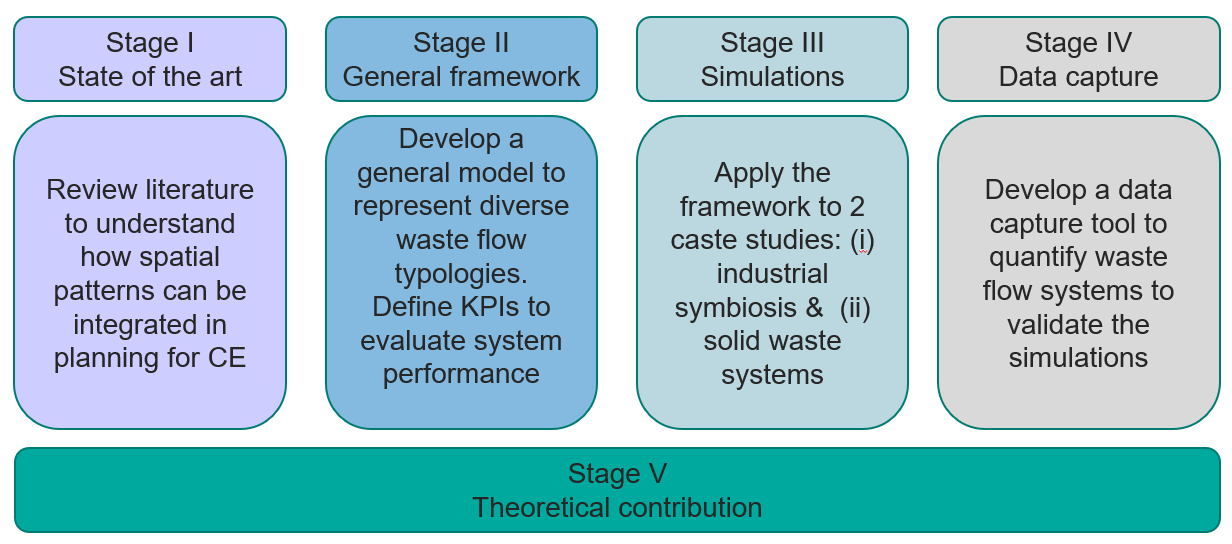
\includegraphics[width=0.8\textwidth]{sections/asset/stage.PNG}
    \caption{Details of stages of research}
    \label{fig:research1s}
\end{figure}

% -	This project is composed by 4 main sequential components and an optional 5th part, that will only be included if there is space to pursue it or it becomes clear that is a critical part of the project. \par
% -	In what follows in this section, I will be describe in greater detail the activities that will be executed in each component and how these components are connected to each other. \par
% -	These components were identified as necessary components to bring unambiguous answers to the main research question faced in this project.  \par
% -	This main question will eventually find partial solution at the end of this project and all the throughout the project different knowledge blocks will be built to reach to these objectives. \par
% -	Based on the identify problem and knowledge gap, the first main objective is to develop a data model capable of modelling how resources flow in a city region. \par
% -	Only then, it would be able to scrutinize the role of the location in closing the loop of resources. v
% -	The rest of this section describes in greater detail each of these four components. \par

\section{Stages of research}
The research has been divided 5 stages, of which 4 of them contribute to feed a fifth stage, that ultimately will use the main learning's from the previous stages. In this last stage the main research question will be addressed and where the main theoretical contributions will be made. During the first stage of the research mainly a literature review will be conducted. Once the marginal curve of leaning starts to flatten work towards a general framework of waste fluxes will start. As the general framework starts too become more stable and there is more certainty that it could be used for simulating different scenarios, the development of these scenarios will start. In parallel to this stage data structures are going to be explored and potentially collected. After the simulation and data capture stages are completed, the model of waste flows will be explored to further understand the role of location patterns to enhance circular economy at different geographical scales. 



In order to further comprehend how these stages relate to each other and how this research is going to progress see the diagram and the subsections below.

\begin{figure}[h!]
    \centering
    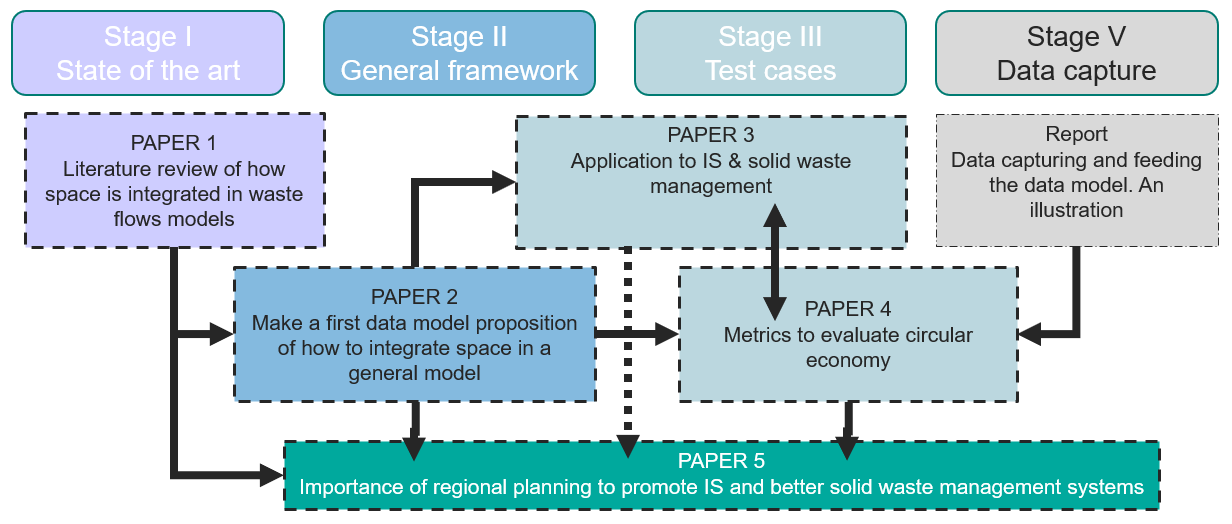
\includegraphics[width=0.8\textwidth]{sections/asset/stage2.PNG}
    \caption{Stages of research, interactions and outputs}
    \label{fig:research2}
\end{figure}






\subsection{Stage 1: Status-quo of modelling waste flows and measuring progress in circular economy processes}
The first stage of the project consists in gaining a better understanding of the concepts of circular economy, urban metabolism, industrial ecology (symbiosis) and municipal solid waste. After gaining more knowledge in these main fields, more specific exploration will be conducted to understand how space (location of socioeconomic activities) has been taken into account to describe and evaluate circular economy performance in city-regions. \par
In this case the objective is to comprehend to what extent space has been integrated into urban metabolism and circular economy ideas. Since one of the distinct attributes of cities and regions, is that these entities are spatial (as geographical), to describe them and to evaluate their performance space must be also considered.  \par
The output of the stage will be to reflect critically about sustainability, planning, circular economy, smart cities and other major concepts that will be referenced in this project. More specific, after the readings, it will become much more clear how space has been used to evaluate circular economy practices in the urban and regional domains. In order to tackle this tasks, an annotated bibliography will be written to highlight and pick major advances in these fields. \par
For this stage, Google Scholars, Scopus and Web of Science will be used to create a database of references to be studied and analyzed. This stage finishes with a deliverable that will be a publishable review that will highlight the need to incorporate space into these domains.\par



% •	Other deliverables: \par

% \begin{enumerate}
%     \item Table with circular economy metrics that take into consideration space 
%     \item Table of waste flow models that consider space
%     \item Simulations and models of waste flows
%     \item Stakeholders
%     \item Potential data providers 
%     \item Set of case studies
%     \item Important parameters
% \end{enumerate}


•	Research questions: 1.1 - 1.2 - 1.3    


\subsection{Stage 2: Design \& development of general framework the flow of secondary resources (waste)}
Towards the end of the second stage, it will be become more clearer how spatial patterns of activities have been modelled and taken into consideration to describe these urban systems. Moreover it will become clearer to what extent the location of activities has been taken into account to evaluate progress in circular economy.
Once it becomes clear how space has been taken into account in previous studies a general framework to study waste fluxes will be proposed.\par
This is a core part of the research since in order to study under a quantitative perspective the role of space and consequently the role of urban (and regional) planning, an operational framework would be needed. This framework will need to be prepared so that is could be populated with case studies and system properties. Open source and transparency of the framework are and performance will be studied. This part of the research requires the part above to be finalized and consequently it would be the point of departure to build the data model that will help up to represent how waste resources (secondary resources) flow in a city-region.\par
Departing from the knowledge gain from the previous stage during this stage a proto-model or conceptual framework will be developed. In order to do this, a clear map of the agents, its properties, how they relate and their action sets should be stated. Once this architecture is defined, the next step is to digitize on one hand the dynamic model, but also a relational data base, so that different case studies could be populated and evaluated. After the proto-model and conceptual framework become stable, this concepts will be digitized using R/PYTHON or a ABM Platform such as Eclipse or Net Logo\par
This stage is a core one, and it is expected that after completion two papers are in condition of being published. It is expected an article that shows the conceptual framework and proto-model comparing different waste cases and indicating potential uses. \par
•	Research question: 2.1 - 2.3 \par


\subsection{Stage 3: Test framework to evaluate solid waste management and Industrial symbiosis}
The conceptual framework is digitized and ready to be tested using different applications. These applications are case studies in different geographical areas and dealing with solid waste management and industrial symbiosis. The specificity of these case studies will depend on the data available for use. These case studies or applications will be used to populate the model. In this stage the model usefulness will be tested. By using the framework with these two waste systems the framework generality and usability will be stressed. As the model is being used and evaluated, there might be a need to change or re-think parts of the model. There will be interactions between this stage and the previous one.  \par
In order to progress in this stage, simulations and data acquisition of industrial symbiosis and solid waste management will be needed. Process the information so that can be integrated in the framework developed in the previous stage. Describe the system properties and evaluate how it is performing based on a set of KPIs. Define a set of scenarios to be modelled. \par
•	Research question: 1.2 - 2.1 - 2.3           \par

\subsection{Stage 4: Data capture and analysis to quantify and map solid waste generation}
This stage will be characterized by using existing data or developing methods to capture information about specific waste materials. By designing, developing or implementing a method to capture and analyze existing data about generation of waste it will be possible to produce tools to be used by practitioners. This will allow municipalities, collection services and recycling facilities to use this information to enhance the provision of those services.      \par
•	Research question: 3.1           \par



\subsection{Stage 5: Theory building, understanding the contribution of spatial planning to promote circular economy practices}
Finally, progress about metrics, models and data will allow to better understand how space determines Circular Economy practices. By combining these leanings, urban and regional planning tools could be used as a tool to promote Circular Economy practices a set of scenarios will be constructed for the two case studies. The idea of scenarios is intrinsic in planning practice and to elucidate what changes in spatial patterns should be promoted, consequently should be  important to run different scenarios and test different hypothesis. \par
This last stage of the research will be conceptual and it will be mainly aimed to contribute to build theory to bridge between urban and regional planning and environmental sciences. This publication would be pursued, only once the previous stages of the research are completed and only then, with the evidence of this project, attempt to bring some answers to general question that this project is trying to reveal. \par
•	Research question: 4.1 - 4.2 - General research question        \par
























% %%%%%%%%%%%%%%%%%%%%%%%%%%%%%%%%%%%%%%%%%%%%%%%%%%%%
% \chapter{Research Methodology and Description}
% %%%%%%%%%%%%%%%%%%%%%%%%%%%%%%%%%%%%%%%%%%%%%%%%%%%%
% This section details the specific methods and materials that will used in order to bring answers to the sub questions stated above. It is expected that by isolating these questions and answer them, an answer to the general research question will emerge. Taking as a starting point, an specific methodological tool set are selected. \par

% For each question try to fill the following form:

% %\textbf{\begin{itemize}
% %    \item Related Literature
% %    \item Data Set
% %    \item Methodology
% %    \item Plan
% %    \item Expected results 
% %\end{itemize}}


% (each sub section should be a task)
% (here is more about tasks)
% (results)


% \section{ Some thoughts on tasks:}

% \textbf{Review to understand}
% -Describing the system, "mapping" it, including space.
% - Identifying and describing in more detail subsystems for further work: IS and household/municipal

% \textbf{Review to assess}
% - Assessing the performance of the waste system: KPIs
% - Assessing the performance potential of the system from a CE perspective: building resilience, characteristic that will predispose it to perform well.

%  \textbf{The data gap issue}
% - Data can be inferred/potentials estimated (see IS work); 
% - data can be simulated based on model of the system; 
% - data can be collected (based on data model): "manually" by actors, or digitally by systems.
% - some empirical data useful to calibrate/validate the simulation and the inferences.
% - real data is necessary for calculating KPI

%  \textbf{The model}

% \textbf{The planning issue}
% - potential/inference/statistics/analysis is necessary for planning guidance towards KPI. What measures should one take with the limited resources and time? To examine the baseline and test scenarios. 



% \section{Metrics and key performance indicators}


% \begin{figure}[h!]
%     \centering
%     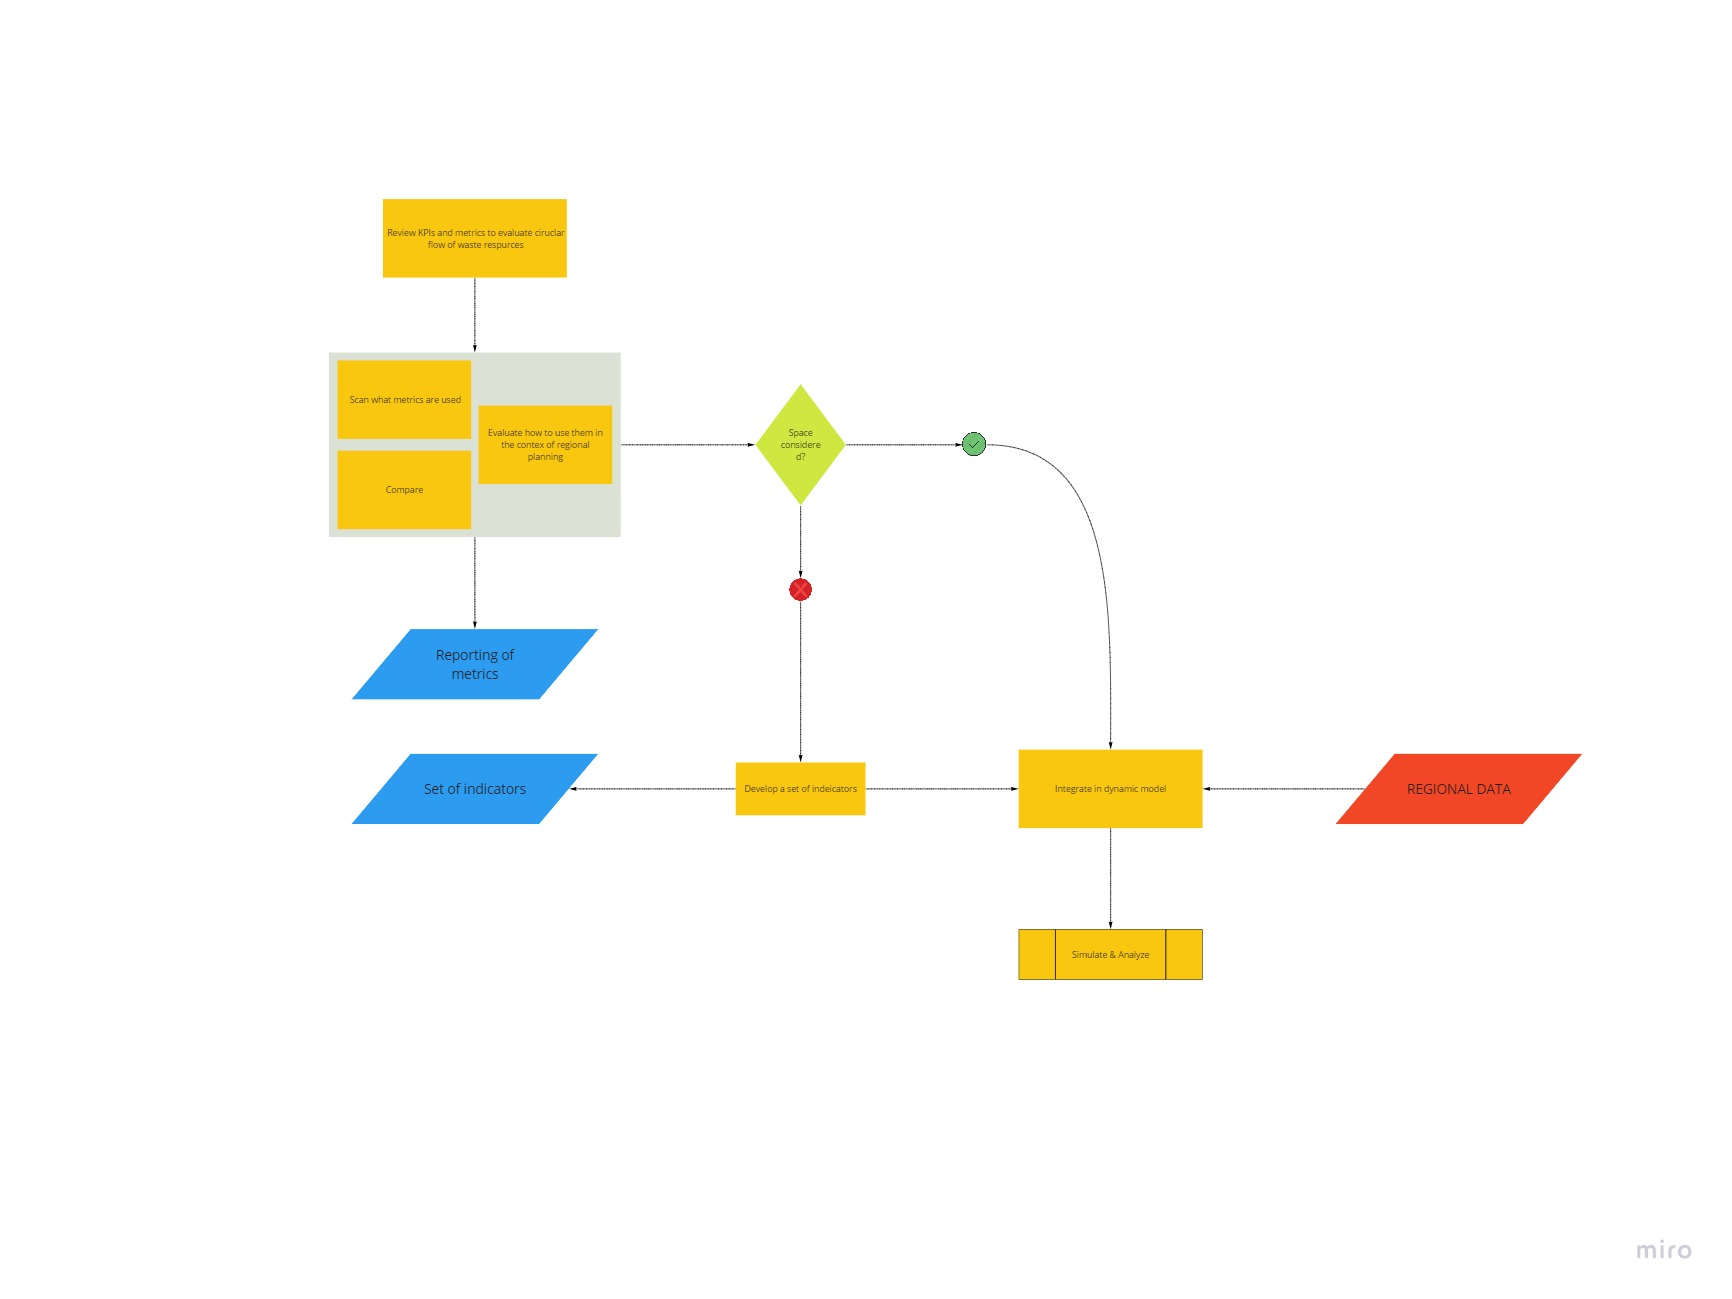
\includegraphics[width=0.8\textwidth]{sections/asset/PHD2 tasks - Metrics exploration.jpg}
%     \caption{Task and workflow for metrics exploration}
%     \label{fig:phd1}
% \end{figure}


% \subsection{State of the art}


% \subsection{Incorporate space into metrics}



% \subsection{Test metrics in models}


% \section{Data capture and processing}



% \begin{figure}[h!]
%     \centering
%     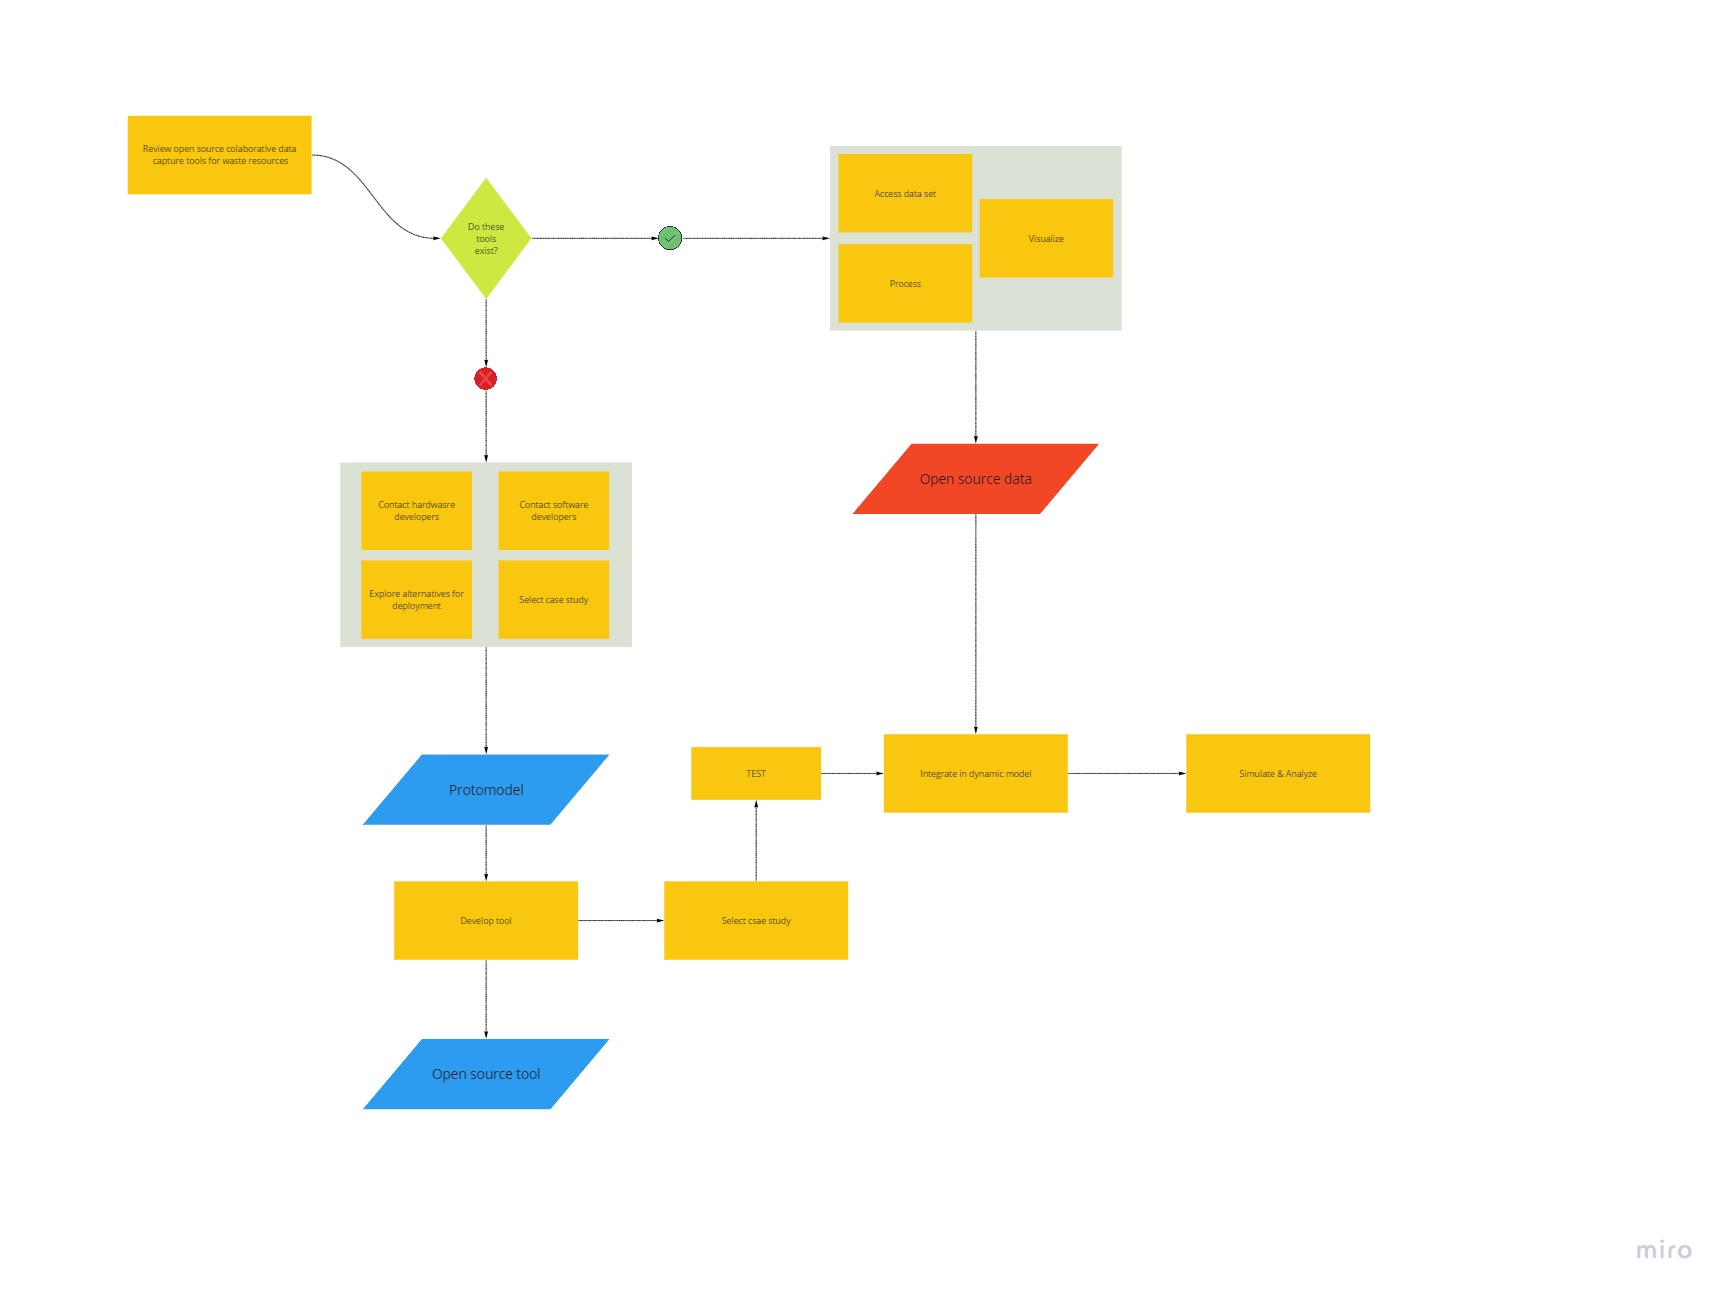
\includegraphics[width=0.8\textwidth]{sections/asset/PHD1 tasks - Data capturing workflow.jpg}
%     \caption{Task and workflow for metrics exploration}
%     \label{fig:phd2}
% \end{figure}
% \subsection{State of the art}

% \subsection{Feed a data model}


% \subsection{Analyze preliminary results and indicate future research}


% \section{Models}


% \begin{figure}[h!]
%     \centering
%     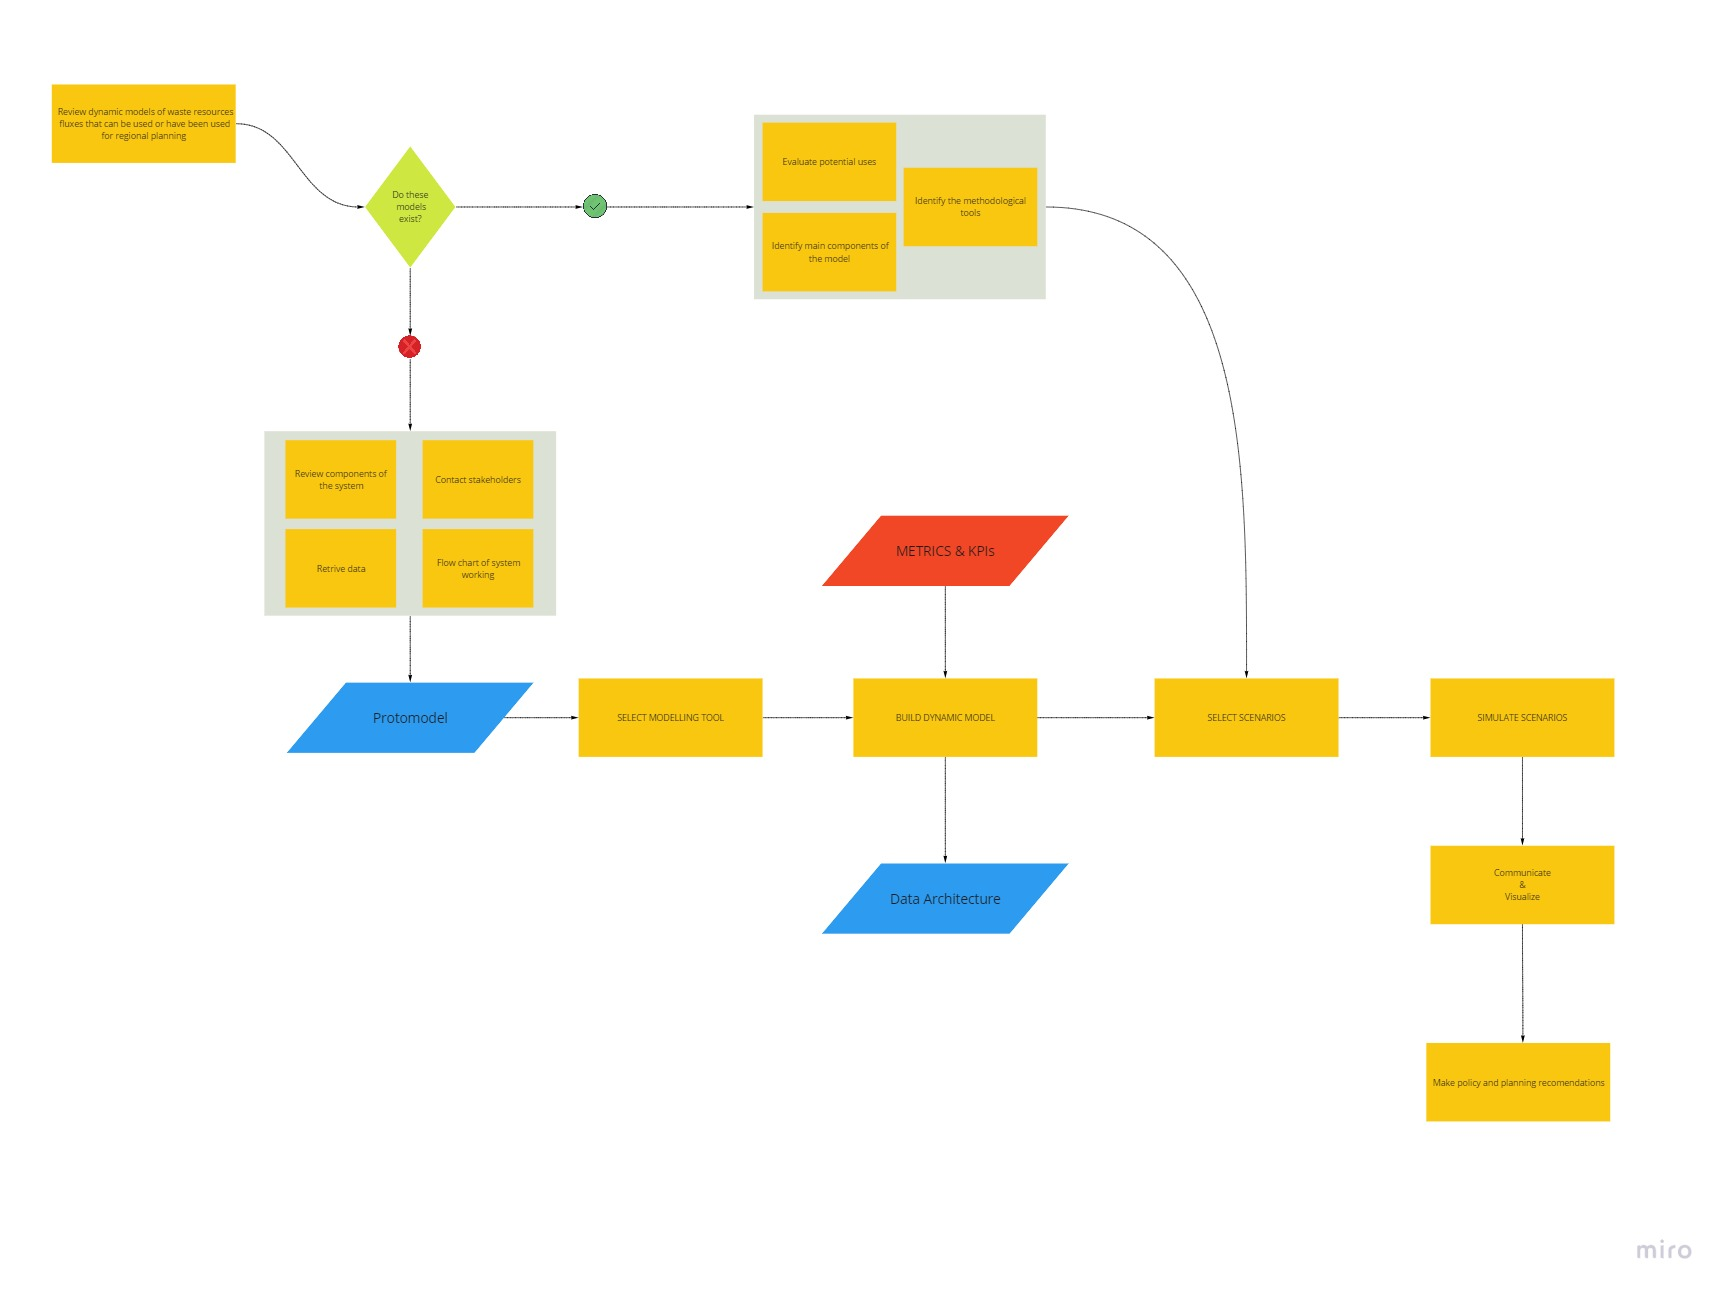
\includegraphics[width=0.8\textwidth]{sections/asset/PHD3 tasks - Modelling workflow.jpg}
%     \caption{Task and workflow for metrics exploration}
%     \label{fig:phd3}
% \end{figure}
% \subsection{State of the art}




% %%%%%%%%%%%%%%%%%%%%%%%%%%%%%%%%%%%%%%%%%%%%%%%%%%%%
% \section{How is the flow of waste resources in a city-region being assessed and what key performance indicators are calculated in order to evaluate how sustainable waste materials flow in a region?}\par
% %%%%%%%%%%%%%%%%%%%%%%%%%%%%%%%%%%%%%%%%%%%%%%%%%%%%

% The aim of this component is to explore the literature of Industrial Symbiosis in search for regional indicators that capture the environmental performance. As seen in the problem definition, in the field of Industrial Symbiosis, space have been omitted and instead a-spacial material flow diagrams have been used to describe the performance of industrial exchanges.  \par

% For this component a literature review will be pursed to better understand how space and urban planning have been addressing the use of waste materials and what key performance indicators should be taken into account to design healthier regions?\par

% In this case, the underlying hypothesis is that space, the specific location of economic activities have not been adequately addressed in the field of Industrial Symbiosis and consequently, the Key Performance Indicators are not suitable to inform regional design practices. \par

% As a result, this component will extract what is the current state of the art to evaluate how sustainable waste resources are flowing in a city-region.\par 

% %%%%%%%%%%%%%%%%%%%%%%%%%%%%%%%%%%%%%%%%%%%%%%%%%%%%
% \section{What can be learn by reviewing well documented case studies? How would a model that captures the flow of waste materials in a region should look like?} \par
% %%%%%%%%%%%%%%%%%%%%%%%%%%%%%%%%%%%%%%%%%%%%%%%%%%%%


% What information is currently being captured? How is space incorporated in these assessments? What role does it play?\par
% Do conclusions drawn from a-spatial material flow diagrams are still valid if space and the costs of moving residual material are taken into account?

% The aim of this component is to review the existing literature of Industrial symbiosis to capture what key performance indicators are being measured and, if the location of firms - space -, is taken into consideration, what role does it play. Given that the domain of Industrial Symbiosis have been focusing on the flow materials, space and the location of firms have not been taken into consideration. Different performance indicators have been developed to asses the performance of industrial symbiosis exchanges, Sbut still the geographical structure have not been fully incorporated. The lack of desegregated information about individual firms, and the fact that the field of Industrial Symbiosis is heavily rooted/associated with Eco-Industrial Parks, where by construction, all firms are co-located, space has not been perceived as a variable to be taken into consideration. \par 
% In this component, this fact will be exposed by looking at how other researcher have been measuring the performance of Industrial Symbiotic relationships. By incorporating space and costs, adding more complexity can introduce conflicting objectives. 


% %%%%%%%%%%%%%%%%%%%%%%%%%%%%%%%%%%%%%%%%%%%%%%%%%%%%
% \section{How can waste material exchanges between industries in a region be spatially modelled? what key performance indicators can be developed using this model?}\par
% %%%%%%%%%%%%%%%%%%%%%%%%%%%%%%%%%%%%%%%%%%%%%%%%%%%%

% Based on case studies of existing industrial symbiosis and the data set of industrial symbiosis developed by the Urban Metabolism group at Chalmers, extract the main features and characteristics that describe the industrial exchange of waste resources. Using the information extracted, design the logic and the data structure of a model that can be used to capture these exchanges. \par

% To start with, using the location of industries, their material inputs and waste resources output, a geographical model will be developed and a set of performance indicators evaluated under different assumptions. \par

% One the structure of the model is settled, meaning that the attributes and the interrelations of the model are not still changing, the model will then be transferred to an agent-based environment where different fluxes will be simulated to study how the performance indicators change as the parameters of the model exchange.
% The expected result of such a description, will be a platform that allows to model and measure different aspects of industrial symbiosis and asses the performance of different scenarios of exchange.\par

% %%%%%%%%%%%%%%%%%%%%%%%%%%%%%%%%%%%%%%%%%%%%%%%%%%%%
% \section{How should waste materials flow in a region in order to achieve an optimal resource usage? How much would it cost to achieve an optimal flow of waste material at a regional level?}\par
% %%%%%%%%%%%%%%%%%%%%%%%%%%%%%%%%%%%%%%%%%%%%%%%%%%%%
% This question is a theoretical own and the aim here is to develop a best case scenario that will help to benchmark the current situation of the regional exchanges of waste materials. Given, the lack of information about the current state, in this case and Agent Based Model will be explored to simulate possible solutions for industrial symbiosis. Different scenarios will show how to optimise for different key performance indicators.\par

% In order to model regional exchanges of waste resources, SEB data set of firms will be explored. Using some of the knowledge building blocks developed by the group of Water Environment Technology at Chalmers, waste by-product types and quantities will be used. An agent-based modeled will be developed to simulate different combinations of material exchanges. The simulations will track different key performance indicators and solutions that maximise them will be computed. This scenario builder will contribute as a benchmark to what is actually occurring in the territory. \par

% This benchmark will allow regional plans to find a direction to steer their regional policies. 
% As a by-product of this research, the exploration of these solutions will contribute to understand possible conflicts between different objective functions. For instance, Co2 emissions caused by transporting the waste resources to its optimal place of use might be higher than disposing it to the nearest treatment facility. \par

% Finally, but not least by modelling scenarios for different objective functions, the cost for different scenarios can be modelled.\par 

% %%%%%%%%%%%%%%%%%%%%%%%%%%%%%%%%%%%%%%%%%%%%%%%%%%%%
% \section{What are the potential uses of such a model? Can this model structure be also used to model the waste at a city level generated by households and managed by a municipality?}\par
% %%%%%%%%%%%%%%%%%%%%%%%%%%%%%%%%%%%%%%%%%%%%%%%%%%%%
% The aim of this component is to continue exploring the model developed above and exploit it  to understand what if scenarios. The model should be open to modify the location of industries, or locate new facilities. As these modifications are incorporated, it is expected that waste exchanges dynamics will change and eventually have impacts on the performance indicators. \par
% By making these modifications to the current information, hypothetical scenarios contribute to transform the tool into a regional planning tool, that will allow practitioners or policy makers to understand how different spatial configurations perform different. 


% %%%%%%%%%%%%%%%%%%%%%%%%%%%%%%%%%%%%%%%%%%%%%%%%%%%%
% \section{Residential solid waste generation and management}\par
% %%%%%%%%%%%%%%%%%%%%%%%%%%%%%%%%%%%%%%%%%%%%%%%%%%%%

% These components, 
% %%%%%%%%%%%%%%%%%%%%%%%%%%%%%%%%%%%%%%%%%%%%%%%%%%%%
% \subsection{Does waste sorting and collaboration with urban recyclers improve the efficiency of urban solid waste management systems}\par
% %%%%%%%%%%%%%%%%%%%%%%%%%%%%%%%%%%%%%%%%%%%%%%%%%%%%




% %%%%%%%%%%%%%%%%%%%%%%%%%%%%%%%%%%%%%%%%%%%%%%%%%%%%
% \section{How to capture information about the amount and quality of waste generated in residential zones?}\par
% %%%%%%%%%%%%%%%%%%%%%%%%%%%%%%%%%%%%%%%%%%%%%%%%%%%%

% The aim of this component is to develop and open source tool to quantity and characterise waste generated by households. By developing a smart bin and providing an specific data feed pipeline, individual household data can be collected, aggregated and processed to inform the waste collection system.
% Moreover it will contribute to provide a systematic methodology of measuring waste, using a smart bin will guaranty that the information is collected in a systematic way IoT will allow to create a network of connected bins that will produce valuable information to enhance waste management capacities. 


% %%%%%%%%%%%%%%%%%%%%%%%%%%%%%%%%%%%%%%%%%%%%%%%%%%%%
% \section{What methods can be used to capture information about the activity of informal recyclers in the context of the global south?}\par


% %%%%%%%%%%%%%%%%%%%%%%%%%%%%%%%%%%%%%%%%%%%%%%%%%%%%
% \section{How can information of collection and generation be integrated and used to enhance the operation of the solid waste management system}\par
% %%%%%%%%%%%%%%%%%%%%%%%%%%%%%%%%%%%%%%%%%%%%%%%%%%%%


% %%%%%%%%%%%%%%%%%%%%%%%%%%%%%%%%%%%%%%%%%%%%%%%%%%%%
% \section{Data model}\par
% \subsubsection{To what extent the industrial symbiosis and residential solid waste system can be captured using the same data model?}\par
% %%%%%%%%%%%%%%%%%%%%%%%%%%%%%%%%%%%%%%%%%%%%%%%%%%%%
